\tikzstyle{arrow} = [thick,->,>=stealth]
    \tikzstyle{cycle} = [
        rectangle,
        minimum width=3cm,
        minimum height=1cm,
        text width=3cm,
        text centered,
        draw=black,
        fill=orange!30
    ]
    \tikzstyle{geste} = [
        rectangle,
        minimum width=3cm,
        minimum height=1cm,
        text width=3cm,
        text centered,
        draw=black,
        fill=green!30
    ]
    \tikzstyle{chanson} = [
        rectangle,
        minimum width=2cm,
        minimum height=1cm,
        text width=2cm,
        text centered,
        draw=black,
        fill=blue!30
    ]
    \tikzstyle{witness} = [
        rectangle,
        minimum width=1cm,
        minimum height=1cm,
        text width=1cm,
        text centered,
        draw=black,
        fill=cyan!30
    ]
    \tikzstyle{doc} = [
        rectangle,
        minimum width=1.5cm,
        minimum height=1cm,
        text width=1.5cm,
        text centered,
        draw=black,
        fill=red!30
    ]
    \tikzstyle{stemma} = [
        rectangle,
        minimum width=3cm,
        minimum height=1cm,
        text width=3cm,
        text centered,
        draw=black,
        fill=yellow!30
    ]
    \tikzstyle{bubble} = [
        circle,
        minimum width=3cm,
        minimum height=1cm,
        text width=3cm,
        text centered,
        draw=black,
        % line width = 0.5cm,
    ]
    \tikzstyle{tinybubble} = [
        rectangle,
        rounded corners,
        minimum width=1cm,
        minimum height=0.5cm,
        text width=1cm,
        text centered,
        draw=black,
        % line width = 0.5cm,
    ]


\begin{frame}{Stemmata}

    Through their instances, both works and texts evolve over time.\\

    \vspace{1em}

    A text evolves through different witnesses.
    A work evolves through different texts.
    Such evolution is described through stemmata.

    \vspace{1em}

    \begin{greenblock}{Stemma}
        Historical text genealogy.

        \centering
        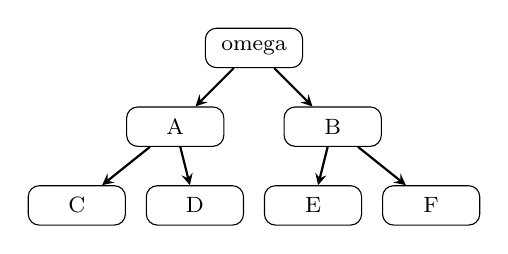
\begin{tikzpicture}
            \node [tinybubble] (omega) {\footnotesize{omega}};
            \node [tinybubble, below of=omega, xshift=-1cm] (a) {\footnotesize{A}};
            \node [tinybubble, below of=omega, xshift=1cm] (b) {\footnotesize{B}};
            \node [tinybubble, below of=a, xshift=-1.25cm] (c) {\footnotesize{C}};
            \node [tinybubble, below of=a, xshift=0.25cm] (d) {\footnotesize{D}};
            \node [tinybubble, below of=b, xshift=-0.25cm] (e) {\footnotesize{E}};
            \node [tinybubble, below of=b, xshift=1.25cm] (f) {\footnotesize{F}};
            \draw [arrow] (omega) -- (a);
            \draw [arrow] (omega) -- (b);
            \draw [arrow] (a) -- (c);
            \draw [arrow] (a) -- (d);
            \draw [arrow] (b) -- (e);
            \draw [arrow] (b) -- (f);
        \end{tikzpicture}
    \end{greenblock}

\end{frame}


\begin{frame}{Text stemmata}

    The \href{https://www.arlima.net/index.html}{Arlima} database has genealogical information available for texts and their witnesses. We can use this information to imitate stemmata.

    \vspace{1em}

    \tiny

    \centering
    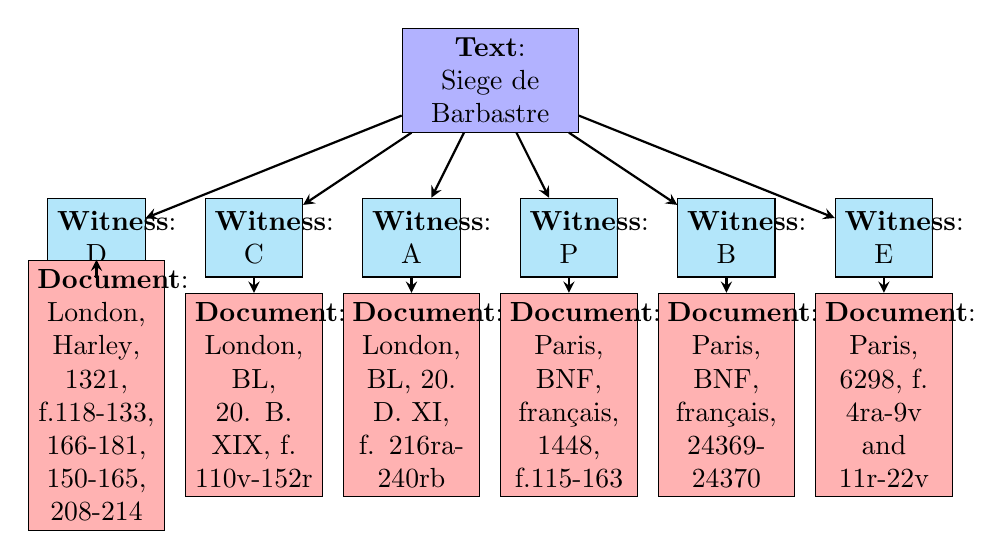
\begin{tikzpicture}[node distance=2cm]

        \node [witness] (witness1) {\textbf{Witness}:\\D};
        \node [doc, below of=witness1] (doc1) {\textbf{Document}:\\London\text{,} Harley\text{,} 1321\text{,} f.118-133\text{,} 166-181\text{,} 150-165\text{,} 208-214};

        \node [witness, right of=witness1] (witness2) {\textbf{Witness}:\\C};
        \node [doc, below of=witness2] (doc2) {\textbf{Document}:\\London\text{,} BL\text{,} 20. B. XIX\text{,} f. 110v-152r};

        \node [witness, right of=witness2] (witness3) {\textbf{Witness}:\\A};
        \node [doc, below of=witness3] (doc3) {\textbf{Document}:\\London\text{,} BL\text{,} 20. D. XI\text{,} f. 216ra-240rb};

        \node [witness, right of=witness3] (witness4) {\textbf{Witness}:\\P};
        \node [doc, below of=witness4] (doc4) {\textbf{Document}:\\Paris\text{,} BNF\text{,} français\text{,} 1448\text{,} f.115-163};

        \node [witness, right of=witness4] (witness5) {\textbf{Witness}:\\B};
        \node [doc, below of=witness5] (doc5) {\textbf{Document}:\\Paris\text{,} BNF\text{,} français\text{,} 24369-24370};

        \node [witness, right of=witness5] (witness6) {\textbf{Witness}:\\E};
        \node [doc, below of=witness6] (doc6) {\textbf{Document}:\\Paris\text{,} 6298\text{,} f. 4ra-9v and 11r-22v};

        \node [chanson, above of=witness2, xshift=3cm] (text) {\textbf{Text}:\\Siege de Barbastre};

        \draw [arrow] (text) -- (witness1);
        \draw [arrow] (text) -- (witness2);
        \draw [arrow] (text) -- (witness3);
        \draw [arrow] (text) -- (witness4);
        \draw [arrow] (text) -- (witness5);
        \draw [arrow] (text) -- (witness6);
        \draw [arrow] (witness1) -- (doc1);
        \draw [arrow] (witness2) -- (doc2);
        \draw [arrow] (witness3) -- (doc3);
        \draw [arrow] (witness4) -- (doc4);
        \draw [arrow] (witness5) -- (doc5);
        \draw [arrow] (witness6) -- (doc6);

    \end{tikzpicture}
    
\end{frame}


\begin{frame}{Text stemmata}

    The \href{https://openstemmata.github.io/index.html}{\textsc{Open Stemmata Project}} maintains a repository of stemma publications,
    which we will leverage to connect texts to witnesses.
    The challenge is linking the witnesses in the Arlima database with those in the Open Stemmata (OP) repository.

    \vspace{1em}

    \centering
    \tiny
    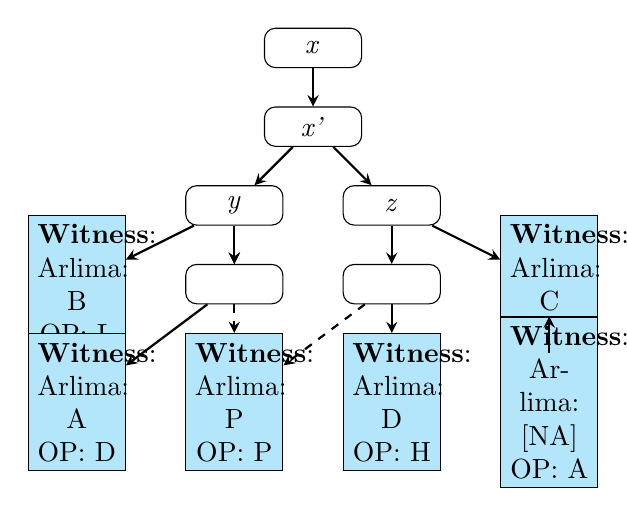
\begin{tikzpicture}[node distance=2cm]

        \node [witness] (witness1) {\textbf{Witness}:\\Arlima: B\\OP: L};
        \node [tinybubble, right of=witness1] (empty1) {};
        \node [tinybubble, right of=empty1] (empty2) {};
        \node [witness, right of=empty2] (witness2) {\textbf{Witness}:\\Arlima: C\\OP: B};

        \node [witness, below of=witness1, yshift=0.5cm] (witness3) {\textbf{Witness}:\\Arlima: A\\OP: D};
        \node [witness, below of=empty1, yshift=0.5cm] (witness4) {\textbf{Witness}:\\Arlima: P\\OP: P};
        \node [witness, below of=empty2, yshift=0.5cm] (witness5) {\textbf{Witness}:\\Arlima: D\\OP: H};
        \node [witness, below of=witness2, yshift=0.5cm] (witness6) {\textbf{Witness}: Arlima: [NA]\\OP: A};

        \node [tinybubble, above of=empty1, yshift=-1cm] (y) {\textit{y}};
        \node [tinybubble, above of=empty2, yshift=-1cm] (z) {\textit{z}};
        \node [tinybubble, above of=y, yshift=-1cm, xshift=1cm] (x1) {\textit{x'}};
        \node [tinybubble, above of=x1, yshift=-1cm] (x) {\textit{x}};

        \draw [arrow] (x) -- (x1);
        \draw [arrow] (x1) -- (y);
        \draw [arrow] (x1) -- (z);
        \draw [arrow] (y) -- (witness1);
        \draw [arrow] (z) -- (witness2);
        \draw [arrow] (y) -- (empty1);
        \draw [arrow] (y) -- (empty1);
        \draw [arrow] (z) -- (empty2);
        \draw [arrow] (witness2) -- (witness6);
        \draw [arrow] (empty1) -- (witness3);
        \draw [thick,dashed,->,>=stealth] (empty1) -- (witness4);
        \draw [thick,dashed,->,>=stealth] (empty2) -- (witness4);
        \draw [arrow] (empty2) -- (witness5);
        
    \end{tikzpicture}

    
\end{frame}